\documentclass[11pt]{ctexart}
\usepackage[utf8]{inputenc}
\usepackage[left=1in,right=1in,top=1.2in,bottom=1.2in]{geometry}
\usepackage{fancyhdr}
\usepackage{amsmath}
\usepackage{amssymb}
\usepackage{multicol}
\usepackage{ctex}
\usepackage{hyperref}
\usepackage{listings}
\usepackage{xcolor}
\usepackage{graphicx,hyperref,url}
\usepackage{minted}
\usepackage{caption}
\usepackage{subfigure}
\usepackage{listings}
\usepackage{color}

\definecolor{dkgreen}{rgb}{0,0.6,0}
\definecolor{gray}{rgb}{0.5,0.5,0.5}
\definecolor{mauve}{rgb}{0.58,0,0.82}

\lstset{frame=tb,
  language=Python,
  aboveskip=3mm,
  belowskip=3mm,
  showstringspaces=false,
  columns=flexible,
  basicstyle={\small\ttfamily},
  numbers=none,
  numberstyle=\tiny\color{gray},
  keywordstyle=\color{blue},
  commentstyle=\color{dkgreen},
  stringstyle=\color{mauve},
  breaklines=true,
  breakatwhitespace=true,
  tabsize=3
}

% \usepackage{titlesec}
% \titlespacing\section{0pt}{15pt}{0pt}
% \titlespacing\subsection{0pt}{5pt}{0pt}
% \titlespacing\subsubsection{0pt}{5pt}{0pt}

\usepackage{enumitem}
\setlist{nolistsep}

\pagestyle{fancy}
\fancyhead[L]{East China Normal University}
\fancyhead[R]{\thepage}
\fancyfoot[C]{}

\fancypagestyle{plain}
{
\fancyhead[L]{East China Normal University}
\fancyhead[R]{\thepage}
\fancyfoot[C]{}
}

\ctexset{section/format=\Large\bfseries}



\setcounter{page}{1}

\title{华东师范大学软件工程实验报告}
\author{谢嘉东\ 10185101247\\陈俊潼\ 10185101210}
\date{March 2020}

\begin{document}

\maketitle

\thispagestyle{empty}

\begin{itemize}
    \item 课程名称:数字图像处理
    \item 年级:2018 级本科
    \item 实验编号:实验 001
    \item 上机实践日期:2020.3
\end{itemize}

\tableofcontents

\thispagestyle{empty}

\newpage

\section{分工情况}

第一次实验相对比较容易,故我们组内两人均完成了实验部分。

实验报告由两人共同撰写。

\section{实验内容}

本实验主要为掌握 PIL 库和 Python 的基本使用方法,含以下内容:

\begin{itemize}
    \item [1] 将 JPG 格式图像文件进行读取和显示。
    \item [2] 将 RGB 彩色图像转变为灰度图像并保存。
    \item [3] 将原图转化为“二值图像”并保存。
    \item [4]将所给的图片尺寸大小分别调整为 $160\times 120$ 、 $320\times 240$ 、 $640\times 480$ ,并对原图进行 $90$ 度和 $180$ 度的旋转变化,将变换后的每个不同结果都保存为 $\text{.PNG}$ 格式。
\end{itemize}

\section{实验目的}

\begin{itemize}
    \item [1] 掌握 PIL 库的基本使用方法
    \item [2] 熟悉 Python 的基本语句和文件相关操作
    \item [3] 理解 RGB 图像在计算机中的存储格式
    \item [4] 理解二值图像、灰度等基本概念
    \item [5] 熟悉 JPG 、 PNG 格式图像的存储方式以及读取方式
\end{itemize}

\section{实验原理}

利用 Python 库 Pillow 中的 PIL 包提供的函数 \mintinline{python}|resize(), point(), thumbnail(), convert()| 等实现各种处理效果,函数的使用方法是:

\begin{itemize}
    \item Image.resize(size, resample=0)
    \begin{itemize}
        \item size – The requested size in pixels, as a 2-tuple: (width, height).
        \item resample – An optional resampling filter. 
    \end{itemize}
    \item Image.point(lut, mode=None)
    \begin{itemize}
        \item lut – A lookup table, containing $256$ (or $65336$ if self.mode==”I” and mode == “L”) values per band in the image. 
        \item mode – Output mode (default is same as input).
    \end{itemize}
    \item Image.thumbnail(size, resample=3)
    \begin{itemize}
        \item size – Requested size.
        \item resample – Optional resampling filter.
    \end{itemize}
    \item Image.convert(mode=None, matrix=None, dither=None, palette=0, colors=256)
    \begin{itemize}
        \item mode – The requested mode.
        \item matrix – An optional conversion matrix. If given, this should be $4$- or $12$-tuple containing floating point values.
        \item dither – Dithering method, used when converting from mode “RGB” to “P” or from “RGB” or “L” to “$1$”. Available methods are NONE or FLOYDSTEINBERG (default).
        \item palette – Palette to use when converting from mode “RGB” to “P”. Available palettes are WEB or ADAPTIVE.
        \item colors – Number of colors to use for the ADAPTIVE palette. Defaults to $256$.
    \end{itemize}
\end{itemize}

\section{实验方法}

\subsection{读取和显示图像}

使用 \mintinline{python}|Image.open()| 函数之后再使用  \mintinline{python}|im.show()| 即可调用系统默认的图像浏览程序打开图片。

  \begin{figure}[htbp]
        \centering
        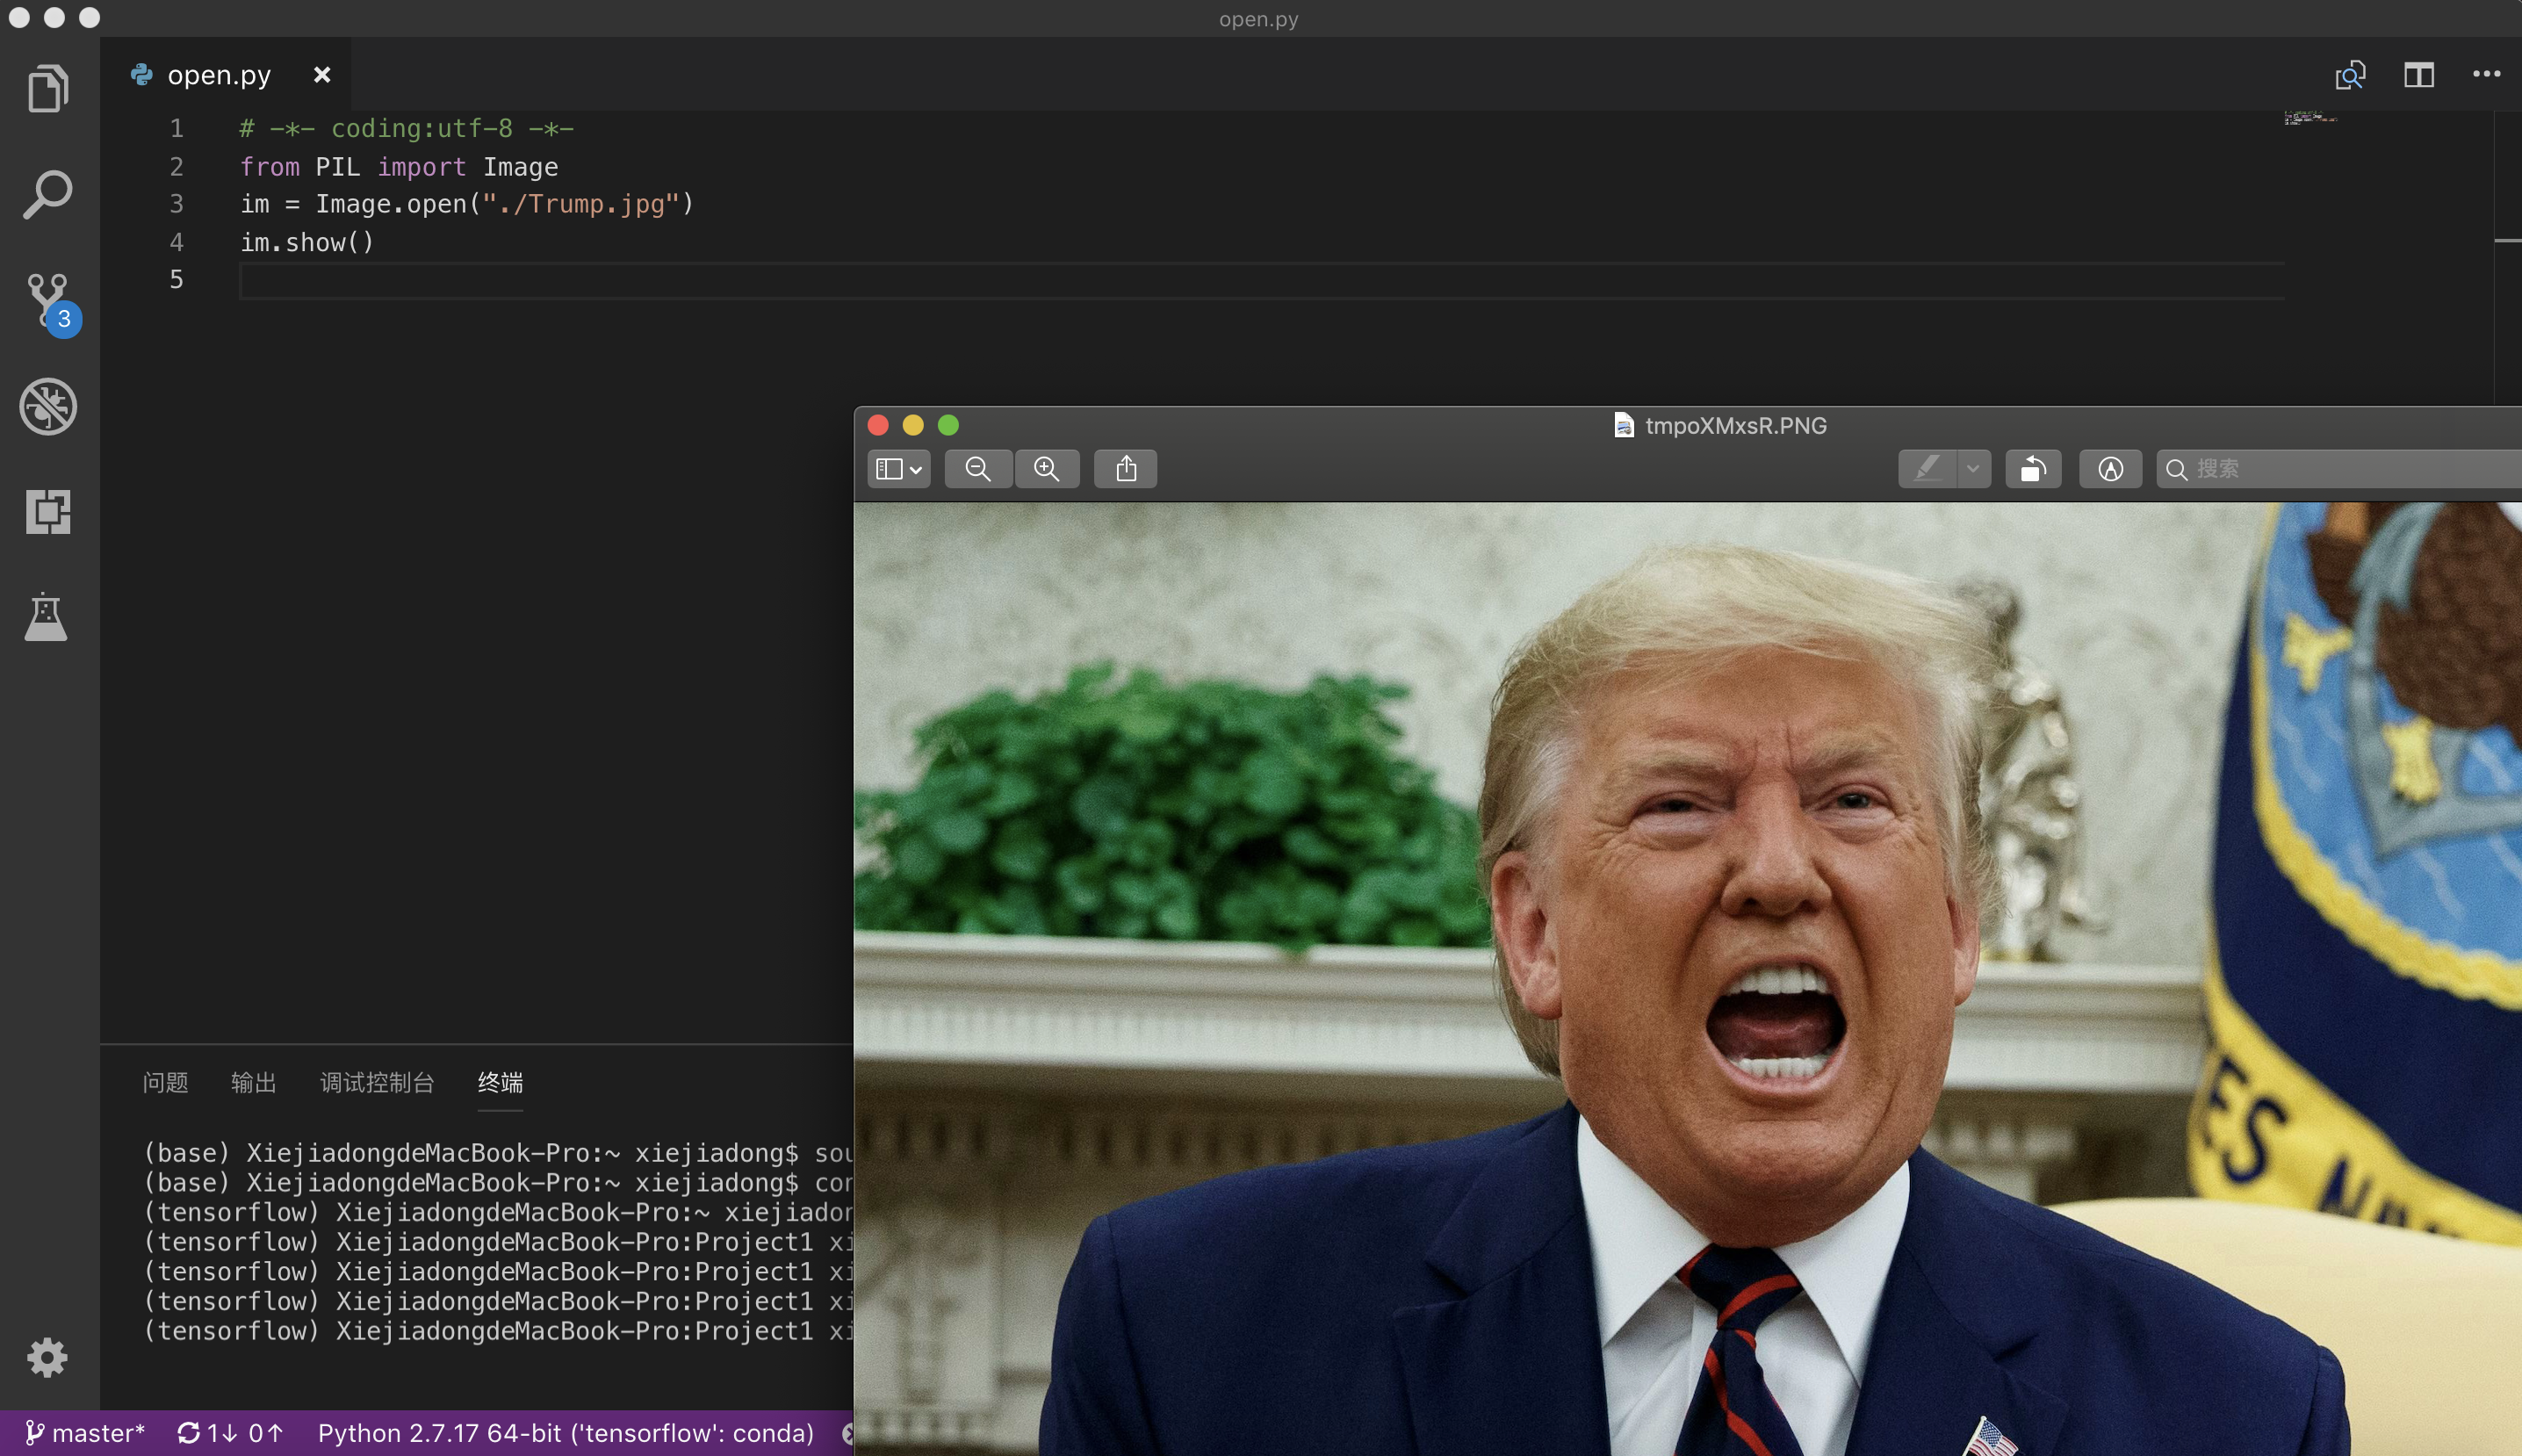
\includegraphics[width=0.6\textwidth]{./pic1.png}
        \caption{读取和显示效果图}\label{fig:digit}
  \end{figure}

\subsection{改变图片形式}

\paragraph{转成灰度图像}

使用 \mintinline{python}|im.convert('L')| 语句即可转成灰度图像。

\paragraph{转成二值图像}

首先将图像转换成灰度图像,再新建一个数组作为映射表。如果色彩深度大于阈值则存 $1$,小于阈值则存 $0$。接着再使用 \mintinline{python}|im.point()| 函数,将映射表传递过去并设置图像模式为二值图像,PIL 库就会逐个遍历像素,将灰度图像的灰度值在数组中映射成 $0$ 或 $1$,最后得到的图像便是二值图像。

实验中我们尝试了不同阀值所带来的效果,最终将灰度值阈值设置为 $110$ ,相对而言可以取得较好效果。

\subsection{改变图片大小与旋转图片}

\paragraph{改变图片大小}

使用 \mintinline{python}|thumbnail()| 函数即可改变图片大小。

\paragraph{旋转图片}

如果是规则的 $90$、$180$、$270$ 度旋转可以直接使用 PIL 库的 \mintinline{python}|transpose()| 函数实现。

之后我们尝试在这一块进行了拓展探究,我们尝试将图片旋转 $45$ 度,但是发现,直接使用 \mintinline{python}|rotate()| 函数进行旋转操作,会导致的图片裁剪。

  \begin{figure}[htbp]
        \centering
        \includegraphics[width=0.6\textwidth]{./Trump_45_bad.png}
        \caption{被裁减的效果}\label{fig:digit}
  \end{figure}

于是,我们探究出了解决这个问题的办法:先用三角函数计算出旋转后并填充黑边的图片大小,新建黑画布,再将原图居中复制到新的画布中,这时使用 \mintinline{python}|rotate()| 就不会将图片裁剪了,结果题便会在实验结果中呈现。

\section{实验结果及分析}

基本完成了实验预期所要达到的要求,并在图片旋转方面,做了一定的拓展实践。

最终的实验结果如下:


  \begin{figure}[htbp]
        \centering
        
\includegraphics[width=0.6\textwidth]{./Trump.jpg}
        \caption{原图}\label{fig:digit}
  \end{figure}
  
    \begin{figure}[htbp]
        \centering
        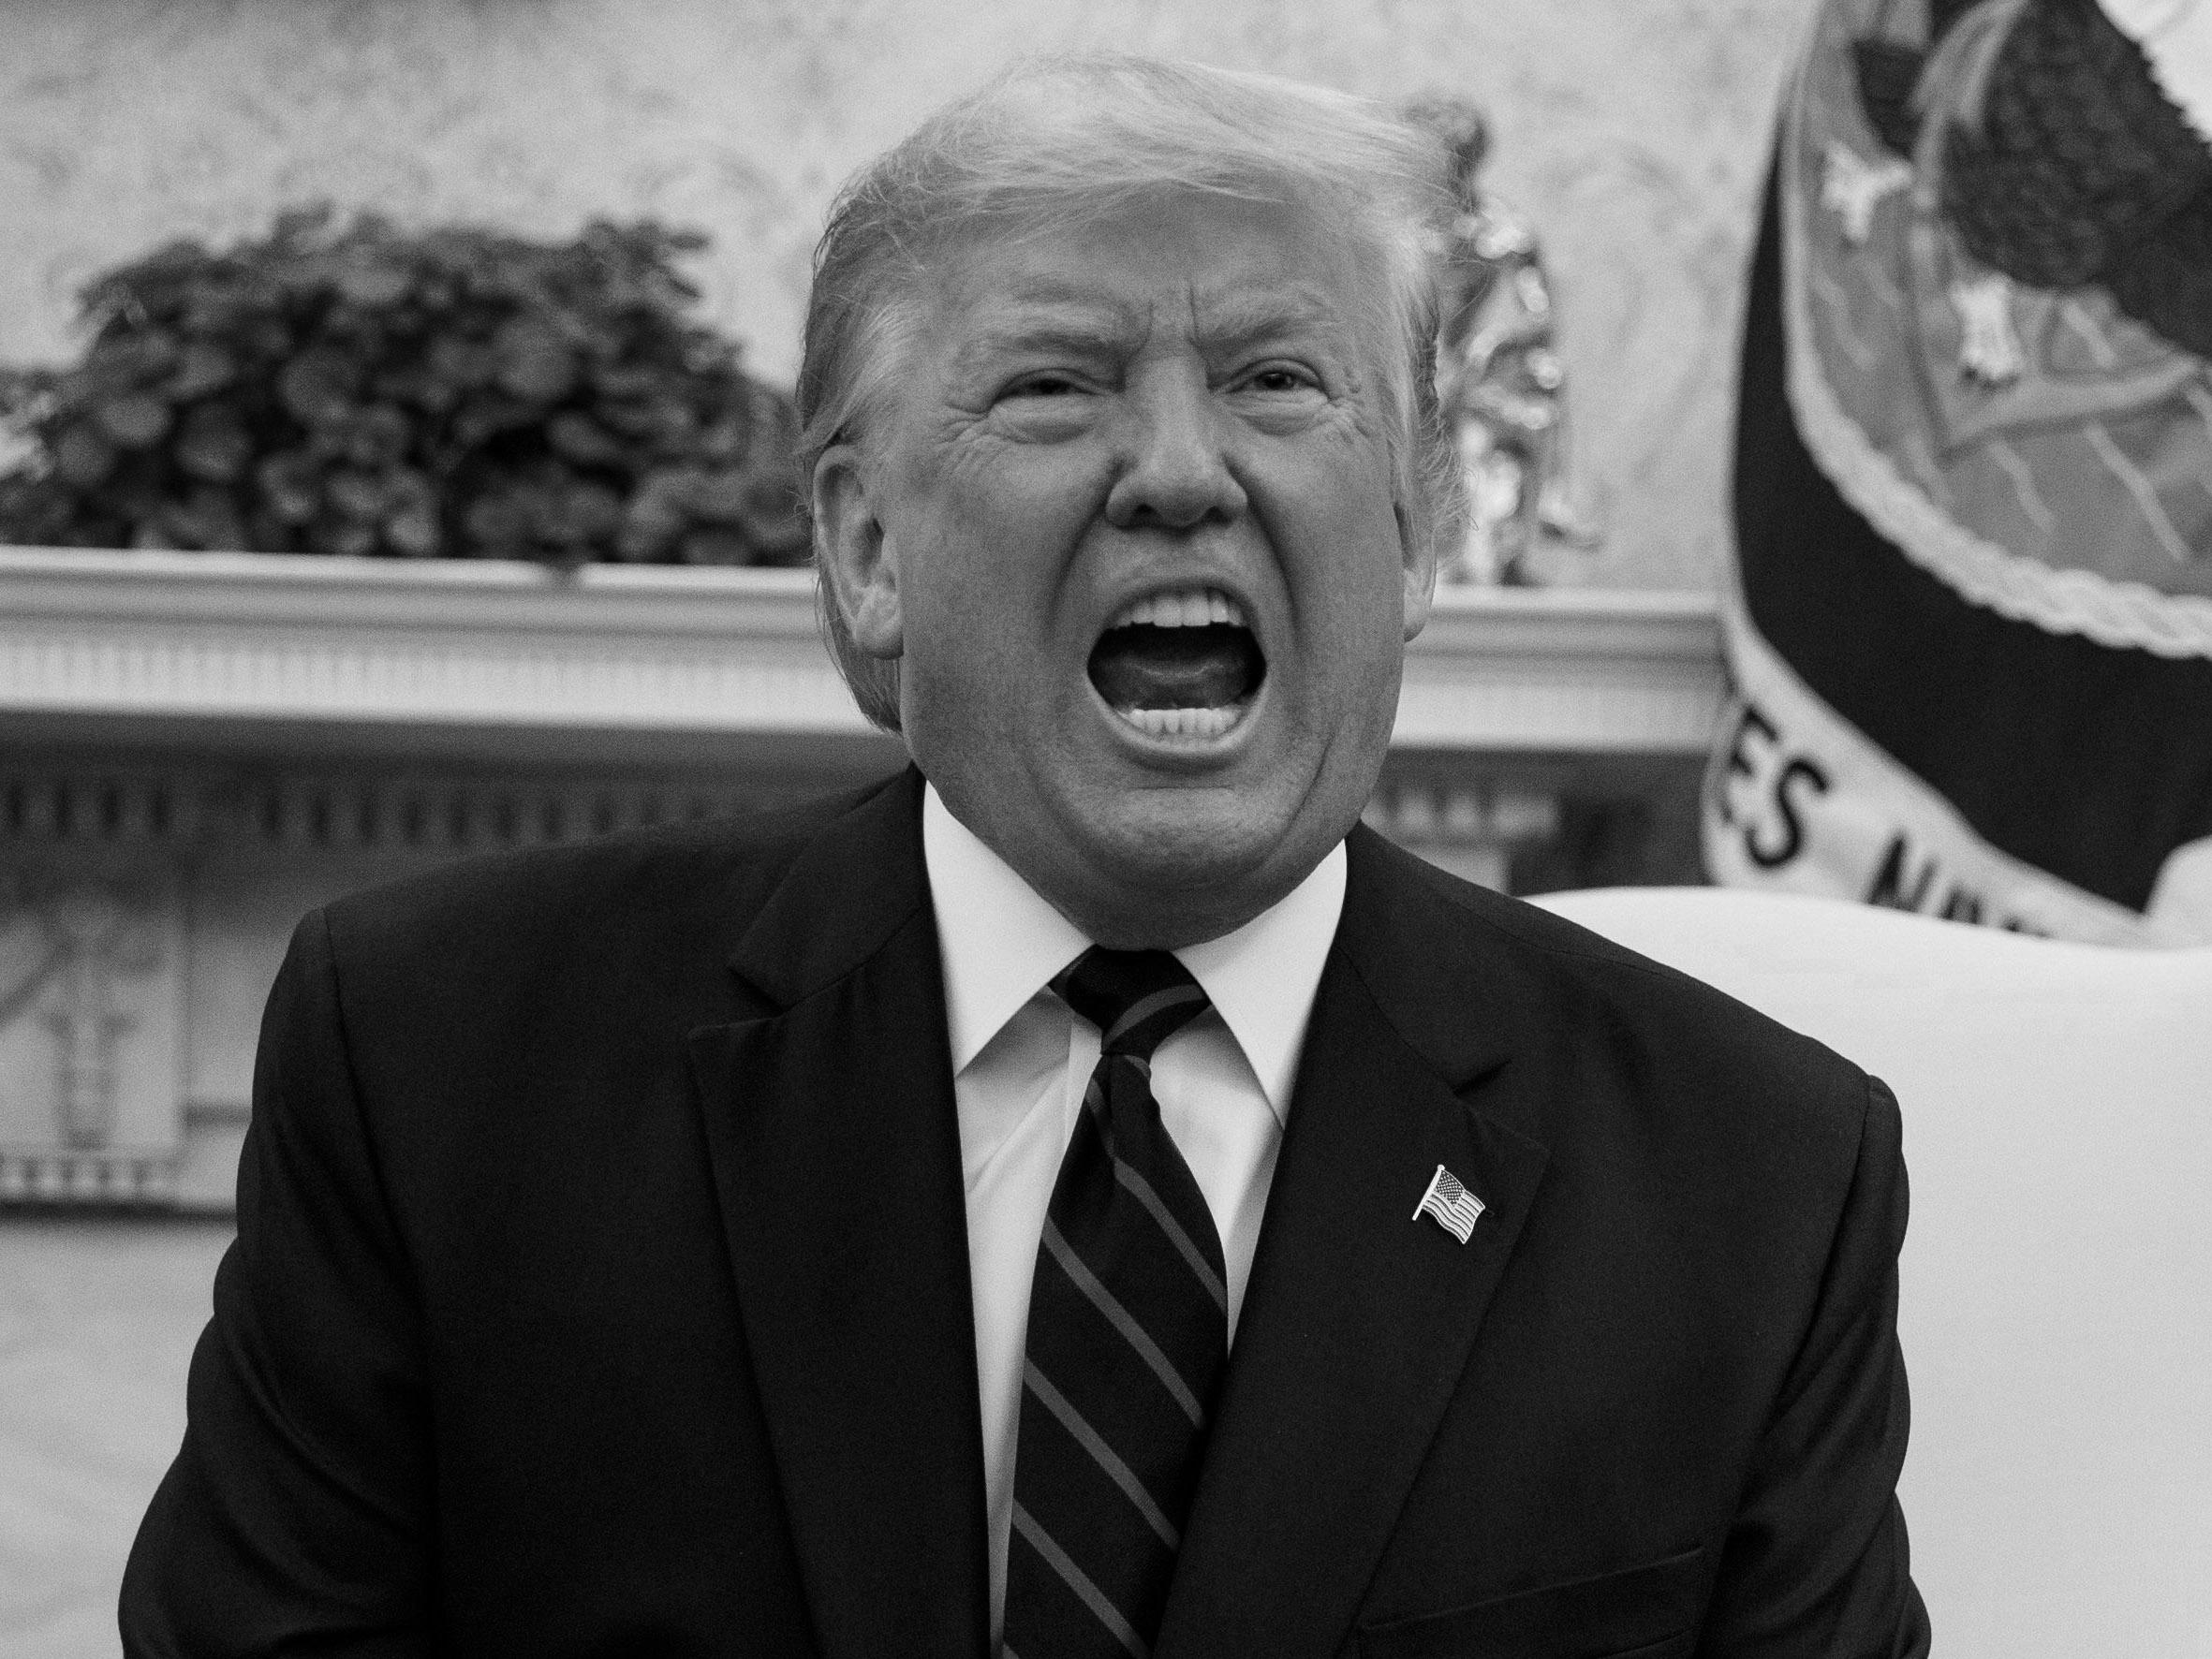
\includegraphics[width=0.6\textwidth]{./Trump_grey.jpg}
        \caption{灰度图像}\label{fig:digit}
  \end{figure}
  
  
    \begin{figure}[htbp]
        \centering
        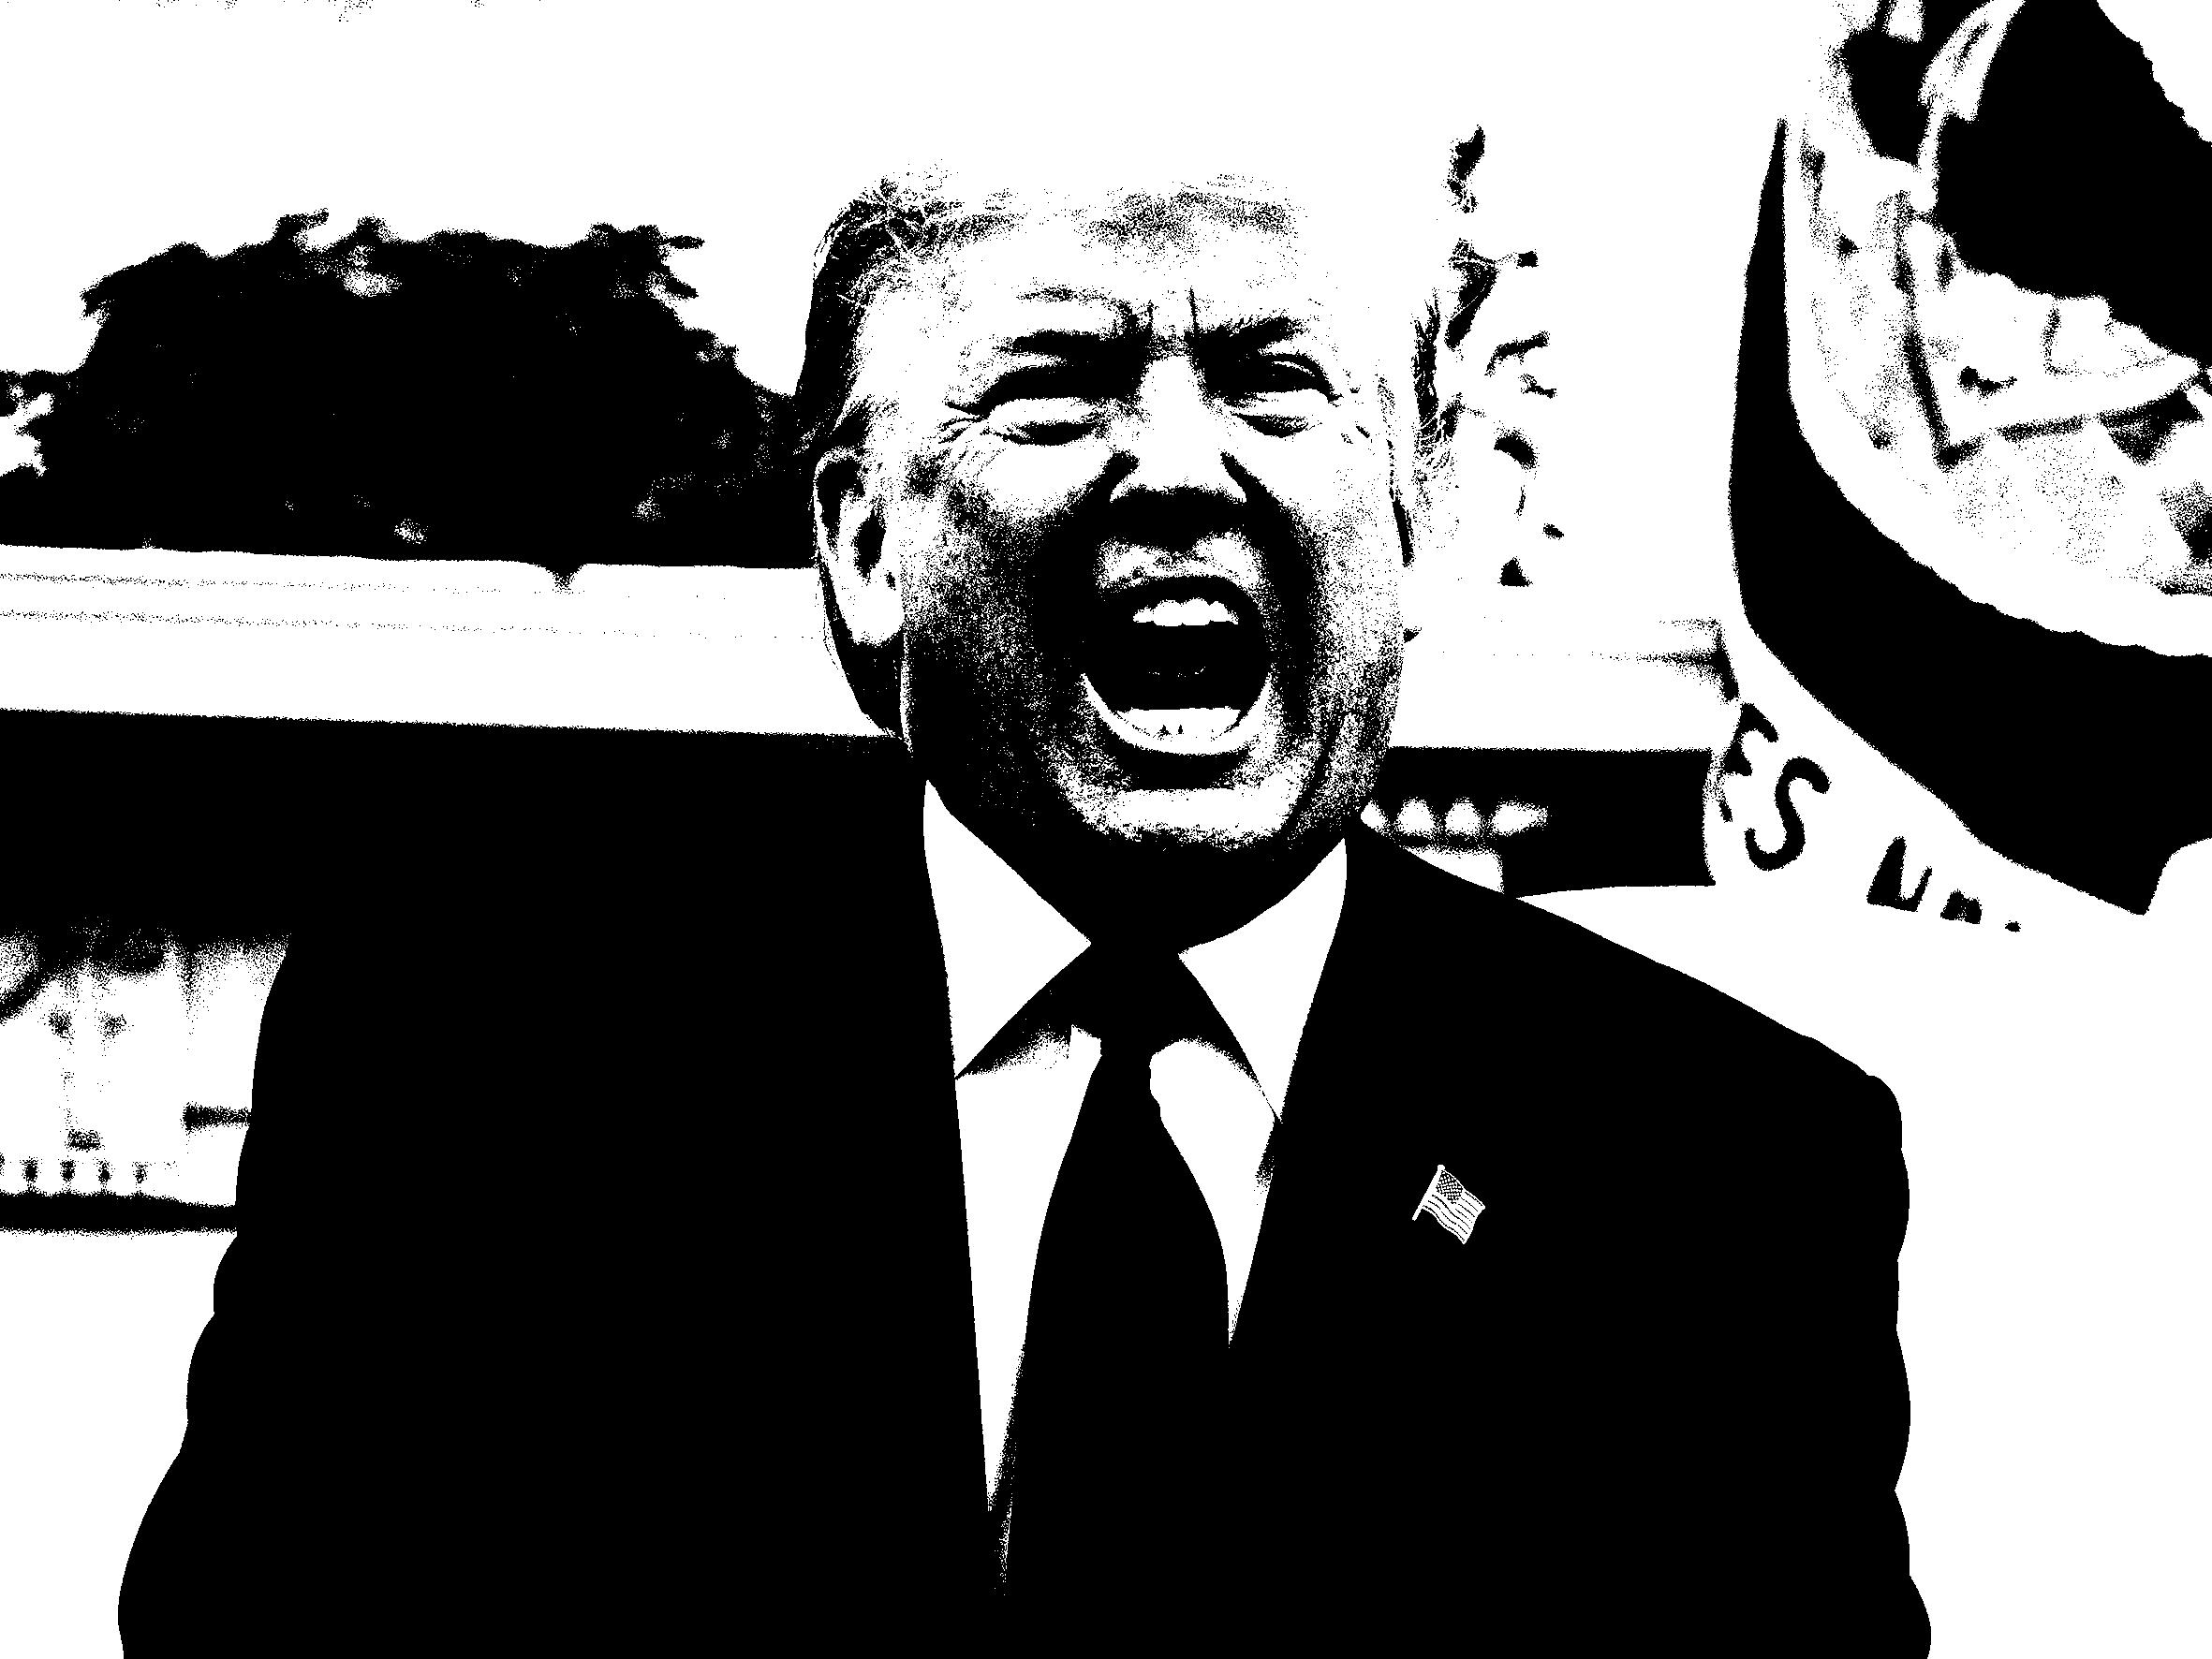
\includegraphics[width=0.6\textwidth]{./Trump_binary_110.jpg}
        \caption{二值图像(灰度阈值 = 110)}\label{fig:digit}
  \end{figure}

\begin{figure}[htbp]

\centering
\subfigure[160 * 120]{
\begin{minipage}[t]{0.3\linewidth}
\centering

\includegraphics[width=0.3\linewidth]{./Trump_160_120.png}
\end{minipage}%
}%
\subfigure[320 * 240]{
\begin{minipage}[t]{0.3\linewidth}
\centering

\includegraphics[width=0.6\linewidth]{./Trump_320_240.png}
\end{minipage}%
}%
\subfigure[640 * 480]{
\begin{minipage}[t]{0.3\linewidth}
\centering

\includegraphics[width=0.8\linewidth]{./Trump_640_480.png}
\end{minipage}
}%
\centering
\caption{缩放图像}

\end{figure}

    \begin{figure}[htbp]
        \centering
        \subfigure[旋转 45 度]{
            \begin{minipage}[t]{0.4\linewidth}
            \centering
            \includegraphics[width=0.8\textwidth]{./Trump_45.png}
        \end{minipage}
        }
        \subfigure[旋转 90 度]{
            \begin{minipage}[t]{0.4\linewidth}
            \centering
            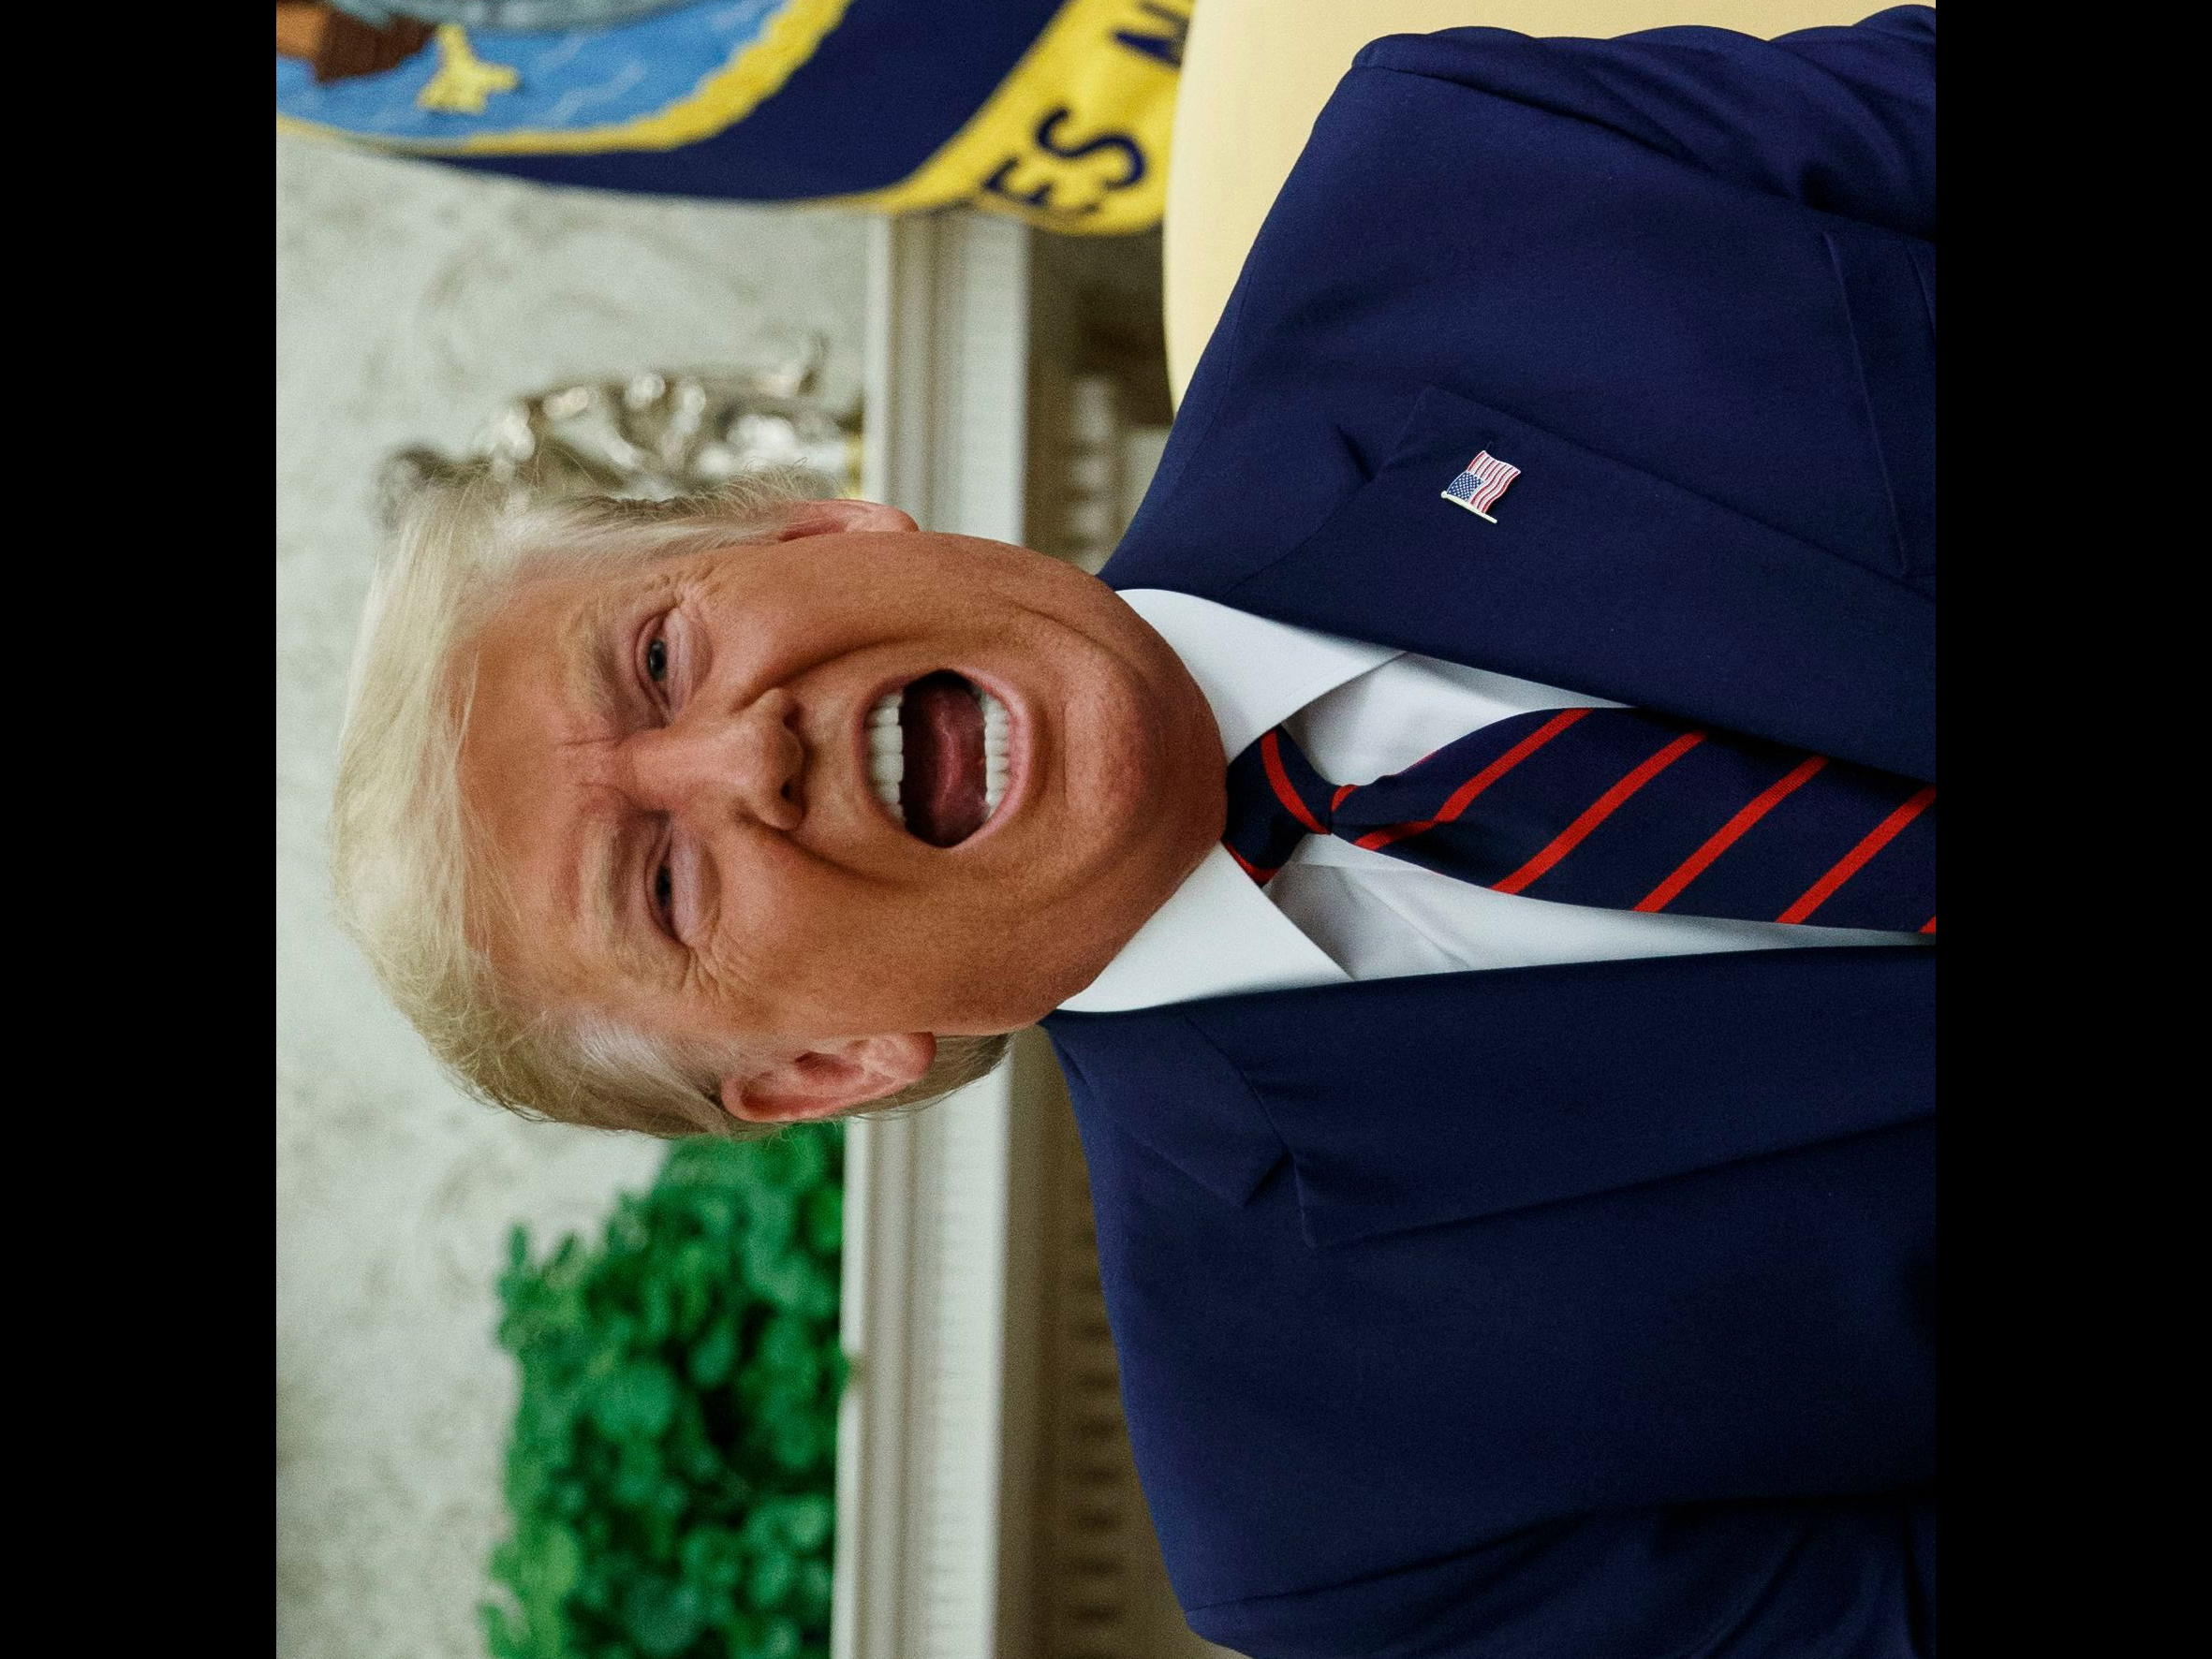
\includegraphics[width=0.8\textwidth]{./Trump_90.png}
            \end{minipage}
        }
        \subfigure[旋转 180 度]{
            \begin{minipage}[t]{0.4\linewidth}
            \centering
            \includegraphics[width=1.0\textwidth]{./Trump_180.png}
            \end{minipage}
        }
        \centering
        \caption{旋转}\label{fig:digit}
  \end{figure}
 
  
\section{主要核心代码}

\subsection{读取与显示图像}

\lstset{language=python}
\begin{lstlisting}
# -*- coding:utf-8 -*-
from PIL import Image
im = Image.open("./Trump.jpg")
im.show()
\end{lstlisting}

\subsection{改变图像形式}

\paragraph{JPG 图片 RBG 模式转灰度模式}

\lstset{language=python}
\begin{lstlisting}
# -*- coding:utf-8 -*-
from PIL import Image
im = Image.open("./Trump.jpg");
#转成灰度图像
im1 = im.convert('L') 
im1.save('Trump_grey.jpg')
\end{lstlisting}

\paragraph{JPG 转二值图像}

\lstset{language=python}
\begin{lstlisting}
# -*- coding:utf-8 -*-
from PIL import Image
im = Image.open("./Trump.jpg")
#转成灰度图像
tmp = im.convert('L')

#设置阀值,大于 threshold 为黑色
threshold = 110
pic = []
#灰度图像每个像素由 0-255 表示
for i in range(256):
    if i < threshold :
        pic.append(0)
    else :
        pic.append(1)
res = tmp.point(pic,'1')
res.save('Trump_binary_110.jpg')
\end{lstlisting}

\subsection{改变图片大小与旋转图片}

\paragraph{调整大小}

\lstset{language=python}
\begin{lstlisting}
# -*- coding:utf-8 -*-
from PIL import Image

outputSize = [
    (320, 240),
    (160, 120),
    (640, 480)
]
im = Image.open("./Trump.jpg");
#改变图片大小
for one in outputSize:
    im.thumbnail(one)
    print(im.format,im.size,im.mode)
    im.save('Trump' + str(one[0]) + '_' + str(one[1]) + '.png')

\end{lstlisting}

\paragraph{旋转图像}

\lstset{language=python}
\begin{lstlisting}
# -*- coding:utf-8 -*-
from PIL import Image
import math
im = Image.open("./Trump.jpg")
# 旋转图片

W = im.size[0]
H = im.size[1]
angle = 45

# 计算旋转后的图片大小
newW = math.cos(math.radians(angle)) * W + math.sin(math.radians(angle)) * H
newH = math.cos(math.radians(angle)) * H + math.sin(math.radians(angle)) * W
out = Image.new("RGB", (int(newW), int(newH)))
box = ( int((newW - W) / 2), int((newH - H)/ 2),  int((newW + W) / 2), int((newH + H)/ 2))
out.paste(im, box)
out = out.rotate(angle)
out.save('Trump_45.png')

spin90 = im.transpose(Image.ROTATE_90)
spin90.save('Trump_90.png')

spin90 = im.transpose(Image.ROTATE_180)
spin90.save('Trump_180.png')
\end{lstlisting}

\section{参考资料}

\begin{thebibliography}{99}

\bibitem{zhao1} Fredrik Lundh,Alex Clark.\\
{\bf Python Imaging Library Reference\\}
{\bf https://pillow.readthedocs.io/en/stable/reference/Image.html\#PIL.Image.Image.point\\}

\bibitem{zhao2} 
大蛇王 (Nick name)\\
{\bf python 图片二值化处理(处理后为纯黑白的图片)\\}
{\bf https://blog.csdn.net/t8116189520/article/details/80271804\\}
\end{thebibliography}

\end{document}
